\chapter{Cơ sở lý thuyết}

Chương 2 trình bày các cơ sở lý thuyết và các nghiên cứu liên quan đến quá trình xây dựng hệ thống.


\section{Tổng quan về Hệ thống Gợi ý}

Hệ thống gợi ý, hay còn được gọi là Recommender Systems - ResSys, được định nghĩa là một phân lớp của hệ thống lọc thông tin, có nhiệm vụ dự đoán mức độ quan tâm hoặc khả năng tương tác của người dùng đối với các thực thể. Dựa trên phương pháp tiếp cận dữ liệu, các hệ thống gợi ý truyền thống và hiện đại thường được phân loại thành ba nhóm chính: Lọc dựa trên nội dung, Lọc cộng tác và Hệ thống lai.

\subsection{Tổng quan về các kỹ thuật gợi ý truyền thống}

Trước sự bùng nổ của các kiến trúc học sâu đa phương thức, hệ thống gợi ý chủ yếu được xây dựng dựa trên hai trường phái tiếp cận cốt lõi: Lọc dựa trên nội dung và Lọc cộng tác. Mỗi phương pháp sở hữu những cơ chế định tuyến độc lập, mang lại những ưu thế riêng biệt nhưng đồng thời cũng bộc lộ những hạn chế mang tính hệ thống.

\begin{figure}[H]
    \centering
    % Khung chứa ảnh 1 (chiếm 45% chiều rộng trang)
    \begin{subfigure}[b]{0.45\textwidth}
        \centering
        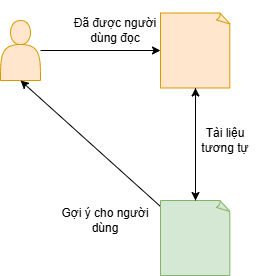
\includegraphics[width=\textwidth]{Images/CBF.png}
        \caption{Lọc dựa trên nội dung.}
        \label{fig:CBF}
    \end{subfigure}
    \hfill % Lệnh này tự động căn đều khoảng trống ở giữa 2 ảnh
    % Khung chứa ảnh 2 (chiếm 45% chiều rộng trang)
    \begin{subfigure}[b]{0.45\textwidth}
        \centering
        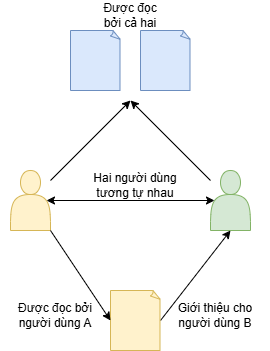
\includegraphics[width=\textwidth]{Images/CF.png}
        \caption{Lọc cộng tác.}
        \label{fig:CF}
    \end{subfigure}
    
    \vspace{0.3cm}
    \caption{Minh họa hai phương pháp gợi ý truyền thống.}
    \label{fig:traditional_methods}
\end{figure}

Phương pháp Lọc dựa trên nội dung, hay Content-Based Filtering, hoạt động dựa trên nguyên lý nhất quán về sở thích cá nhân. Kỹ thuật này trích xuất các đặc trưng nội tại của sản phẩm bao gồm văn bản, danh mục hoặc thương hiệu để xây dựng không gian vector, sau đó tính toán độ tương đồng với hồ sơ sở thích của người dùng \cite{18}. Ưu điểm chiến lược của phương pháp này là khả năng giải quyết triệt để bài toán Khởi động lạnh cho sản phẩm mới. Tuy nhiên, thuật toán sẽ bộc lộ hạn chế trong năng lực phân tích nội dung khi tiếp cận với các mặt hàng yêu cầu cảm nhận chủ quan tinh tế, ví dụ như việc đánh giá mức độ hài hước của hai cuốn truyện cười, hoặc khi xử lý những dữ liệu phi cấu trúc phức tạp như phim ảnh. Đồng thời thuật toán này có hiện tượng chuyên biệt hóa quá mức tạo ra vòng lặp gợi ý nhàm chán và có rào cản khởi động lạnh đối với người dùng mới.

Trái ngược với cách tiếp cận trên, phương pháp Lọc cộng tác, thường được biết đến với thuật ngữ Collaborative Filtering \cite{18}, bỏ qua hoàn toàn nội dung sản phẩm để tập trung khai thác các mẫu hành vi ẩn trong cộng đồng. Dựa trên ma trận tương tác giữa người dùng và mặt hàng, hệ thống áp dụng phương pháp láng giềng gần nhất thuộc nhóm tiếp cận dựa trên bộ nhớ, hoặc vận dụng các kỹ thuật nén không gian ẩn như Phân rã ma trận thuộc nhóm tiếp cận dựa trên mô hình để tìm ra sự đồng điệu về sở thích. Sức mạnh lớn nhất của kỹ thuật này là khả năng mang lại tính khám phá cao, giúp đề xuất những sản phẩm xuyên danh mục một cách chính xác. Mặc dù mang lại hiệu suất vượt trội, sự phụ thuộc tuyệt đối vào lịch sử tương tác khiến Lọc cộng tác hoàn toàn tê liệt trước bài toán Khởi động lạnh cho cả người dùng lẫn sản phẩm mới. Đồng thời, hệ thống sẽ gặp hiện tượng suy giảm hiệu năng nghiêm trọng khi ma trận dữ liệu trở nên quá thưa thớt ở quy mô công nghiệp.

\subsection{Hệ thống Gợi ý Lai}

Sự ra đời của hệ thống gợi ý lai đánh dấu bước phát triển quan trọng nhằm khắc phục các hạn chế cố hữu khi triển khai độc lập phương pháp lọc cộng tác hoặc lọc dựa trên nội dung. Mục tiêu cốt lõi của hướng tiếp cận này là tối ưu hóa hiệu suất dự đoán thông qua việc tổng hợp sức mạnh từ cả dữ liệu hành vi người dùng và các thông tin đặc tả phong phú của sản phẩm. Trong giai đoạn trước khi học sâu trở nên phổ biến, các kiến trúc lai truyền thống thường được áp dụng dựa trên ba chiến lược kết hợp chủ đạo nhằm dung hòa các thuật toán nền tảng.

Đầu tiên là phương pháp lai trọng số, được xem là kỹ thuật cộng gộp đơn giản nhất trong các mô hình lai. Cơ chế vận hành của nó dựa trên việc triển khai song song các mô hình thành phần, sau đó tính toán điểm số xếp hạng cuối cùng bằng tổng có trọng số của các kết quả dự đoán riêng lẻ\cite{18}. Mặc dù ưu điểm là dễ triển khai, phương pháp này gặp hạn chế lớn do giả định mối quan hệ giữa các mô hình luôn là tuyến tính và đòi hỏi quá trình tinh chỉnh tham số thủ công rất kỹ lưỡng để cân bằng hiệu quả giữa các thành phần.

Chiến lược thứ hai là phương pháp lai chuyển đổi, hoạt động tương tự như một cơ chế điều hướng thông minh dựa trên trạng thái dữ liệu thực tế. Hệ thống sẽ linh hoạt lựa chọn thuật toán phù hợp nhất cho từng ngữ cảnh cụ thể, điển hình là việc ưu tiên sử dụng lọc theo nội dung đối với người dùng mới để giải quyết vấn đề khởi động lạnh, sau đó tự động chuyển sang lọc cộng tác khi đã thu thập đủ lịch sử tương tác tin cậy\cite{18}. Tuy nhiên, nhược điểm của chiến lược này nằm ở sự thiếu tính liên tục, dẫn đến trải nghiệm gợi ý có thể bị đứt gãy hoặc thiếu sự mượt mà trong quá trình chuyển giao giữa các mô hình.

Chiến lược kết hợp đặc trưng đại diện cho một bước chuyển dịch quan trọng trong kiến trúc hệ thống gợi ý lai, nơi ranh giới giữa dữ liệu nội dung và dữ liệu hành vi được xóa bỏ để hướng tới một không gian biểu diễn thống nhất. Khác với các phương pháp lai ghép lỏng lẻo như lai trọng số hay lai chuyển đổi vốn xử lý các mô hình thành phần một cách độc lập, phương pháp này chủ động hợp nhất các nguồn thông tin ngay từ giai đoạn đầu vào. Mục tiêu cốt lõi là làm giàu không gian đặc trưng, cho phép thuật toán học được sự tương quan chéo giữa các đặc tính nội tại của sản phẩm với hành vi tương tác của người dùng, thay vì chỉ dựa vào các mã định danh thưa thớt.

Kế thừa và phát triển tư duy này để giải quyết triệt để bài toán khởi động lạnh, Kula\cite{20} đã giới thiệu mô hình LightFM, một kiến trúc lai hiệu quả kết hợp ưu điểm của cả lọc cộng tác và lọc theo nội dung. Điểm đột phá của LightFM nằm ở cơ chế biểu diễn vector linh hoạt, trong đó biểu diễn của một người dùng hoặc sản phẩm được xác định bằng tổng các vector nhúng của định danh và các vector nhúng của các thuộc tính mô tả đi kèm. Nhờ cơ chế cộng gộp này, hệ thống có khả năng suy luận độ tương đồng dựa trên các đặc điểm chung ngay cả khi sản phẩm đó chưa từng có lịch sử tương tác, đảm bảo luồng gợi ý được duy trì liên tục và chính xác cho các thực thể mới.

Tuy nhiên, mặc dù các phương pháp kết hợp đặc trưng như Factorization Machines hay LightFM đã đạt được những thành công nhất định, chúng vẫn tồn tại những hạn chế về khả năng biểu diễn các mẫu dữ liệu phức tạp. Như Cheng và cộng sự\cite{21} đã phân tích trong công trình về kiến trúc Wide \& Deep, các mô hình dựa trên tích vô hướng hoặc biến đổi tuyến tính thường thiên về khả năng ghi nhớ các mẫu đồng xuất hiện trong quá khứ nhưng lại hạn chế trong việc tổng quát hóa các mối quan hệ phi tuyến tính mức cao. Nhận định này đã mở đường cho sự phát triển của các kiến trúc mạng nơ-ron sâu hiện đại, nơi các lớp ẩn đa tầng được sử dụng để trích xuất và kết hợp đặc trưng một cách tinh vi hơn nhằm thấu hiểu sâu sắc ý định người dùng.

\subsection{Hệ thống gợi ý đa giai đoạn}

Trong bối cảnh các sàn thương mại điện tử hiện đại như Amazon, Alibaba hay Shopee đang lưu trữ hàng tỷ sản phẩm, việc xây dựng một hệ thống gợi ý vừa đảm bảo độ chính xác tuyệt đối, vừa đáp ứng được thời gian phản hồi theo thời gian thực là một thách thức cực kỳ lớn đối với các kỹ sư máy học. Nếu sử dụng một mô hình ngôn ngữ sâu sắc và phức tạp để tính toán độ tương quan cho toàn bộ kho dữ liệu mỗi khi người dùng thực hiện truy vấn, hệ thống sẽ gặp phải độ trễ không thể chấp nhận được, gây ảnh hưởng trực tiếp đến trải nghiệm và doanh thu. Để giải quyết mâu thuẫn giữa hiệu năng và độ chính xác, kiến trúc Gợi ý Đa giai đoạn đã ra đời và trở thành tiêu chuẩn công nghiệp phổ biến, giúp tối ưu hóa quá trình xử lý thông qua một cấu trúc hình phễu lọc giảm dần về số lượng nhưng tăng dần về độ tinh vi của thuật toán.

\begin{figure}[H]
\centering
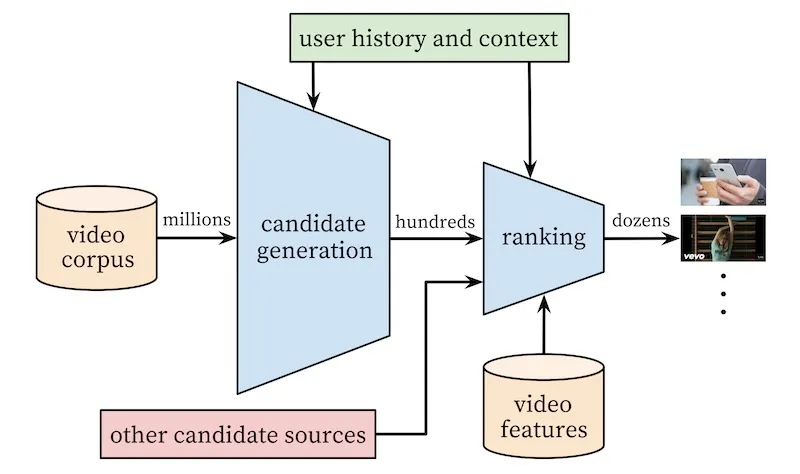
\includegraphics[width=0.85\textwidth]{Images/multi.png}
\vspace{1em}
\caption{Kiến trúc hình phễu tiêu biểu của hệ thống gợi ý đa giai đoạn}
\label{fig:multi_stage_funnel}
\end{figure}

Như hình \ref{fig:multi_stage_funnel}, hệ thống không cố gắng tìm ra kết quả tốt nhất ngay lập tức mà chia quy trình thành các pha tách biệt, trong đó nổi bật nhất là sự phối hợp giữa hai giai đoạn then chốt: Truy xuất (Retrieval) và Xếp hạng lại (Ranking/Reranking). Cách tiếp cận này lần đầu tiên được phổ biến rộng rãi thông qua công trình nghiên cứu kinh điển của Covington và các cộng sự tại Google (2016) về hệ thống gợi ý cho YouTube \cite{9}. Trong nghiên cứu này, các tác giả đã chỉ ra rằng việc sử dụng một mô hình đơn lẻ cho toàn bộ quy trình là không hiệu quả; thay vào đó, hệ thống cần một bộ lọc thô để loại bỏ hàng triệu thực thể không liên quan và những bộ lọc tinh phía sau để sắp xếp các ứng viên tiềm năng nhất vào vị trí hiển thị tối ưu.

Giai đoạn đầu tiên là Truy xuất đóng vai trò như một bộ lọc thô với nhiệm vụ sàng lọc nhanh chóng từ hàng triệu sản phẩm xuống còn khoảng vài trăm ứng viên. Tại giai đoạn này, tốc độ là yếu tố tiên quyết để đảm bảo tính thời gian thực. Kiến trúc chủ đạo thường được sử dụng là Bi-Encoder hay còn gọi là kiến trúc Two-Tower.

Trong kiến trúc này, tháp người dùng và tháp sản phẩm hoạt động độc lập, cho phép hệ thống tính toán trước và lưu trữ các embeddings của toàn bộ kho hàng vào cùng một không gian vector tiềm ẩn. Khi có truy vấn, hệ thống chỉ cần mã hóa câu lệnh người dùng và thực hiện các phép tính đại số đơn giản như tích vô hướng hoặc Cosine Similarity thông qua các thuật toán tìm kiếm ANN. Điểm mạnh của Bi-Encoder là khả năng quét qua hàng triệu thực thể chỉ trong vài mili-giây. Tuy nhiên, do áp dụng cơ chế Late Interaction, nơi truy vấn và sản phẩm không hề trao đổi thông tin với nhau trong quá trình mã hóa, mô hình thường bỏ lỡ các sắc thái ngữ nghĩa giao thoa chi tiết giữa hai đối tượng.

Ngay sau khi có được danh sách ứng viên từ pha Truy xuất, hệ thống chuyển sang giai đoạn Xếp hạng lại để thực hiện những tính toán chuyên sâu hơn trên tập dữ liệu đã được thu hẹp (thường từ vài chục đến vài trăm sản phẩm như mô tả trong sơ đồ hình phễu). Đây là giai đoạn mà độ chính xác được đặt lên hàng đầu nhằm đảm bảo những sản phẩm phù hợp nhất với ý định người dùng và cá nhân hóa sâu sắc sẽ được hiển thị ở những vị trí đầu tiên. Kiến trúc hiệu quả nhất cho giai đoạn này là Cross-Encoder. Khác với Bi-Encoder, Cross-Encoder nhận đầu vào là sự kết hợp đồng thời giữa câu truy vấn và thông tin sản phẩm, cho phép cơ chế Self-Attention của Transformer thực hiện Tương tác sớm. Từng token trong câu lệnh của người dùng có thể soi chiếu và tương tác trực tiếp với từng đặc trưng của sản phẩm ở mọi tầng của mạng nơ-ron. Cơ chế này giúp mô hình nắm bắt được những mối liên hệ ẩn ý, sự tương đồng ngữ nghĩa phức tạp và đặc biệt là khả năng cá nhân hóa dựa trên lịch sử hành vi mua sắm. Việc áp dụng Cross-Encoder ở giai đoạn Reranking giúp hệ thống đạt được sự tối ưu về mặt chất lượng, vì lúc này mô hình chỉ phải xử lý một lượng nhỏ ứng viên, cho phép sử dụng các kiến trúc nặng nề và phức tạp mà vẫn đảm bảo thời gian phản hồi tổng thể.

Sự kết hợp giữa Two-Tower và Cross-Encoder tạo nên một hệ chỉnh thể hoàn chỉnh, giúp hệ thống gợi ý vừa có thể quét qua quy mô dữ liệu khổng lồ, vừa có thể đưa ra những đề xuất mang tính cá nhân hóa cao độ. Kế thừa và tuân thủ trọn vẹn triết lý đa giai đoạn đó, đồ án này tiến hành triển khai kiến trúc Bi-Encoder làm nền tảng cho giai đoạn Truy xuất nhằm khoanh vùng tập ứng viên nhanh chóng, và áp dụng mô hình Cross-Encoder được tích hợp thêm các thành phần bổ trợ cho giai đoạn Xếp hạng lại. Việc ứng dụng cơ chế này ở pha cuối đóng vai trò như một mảnh ghép chiến lược, bởi nó không chỉ giữ được sức mạnh tương tác ngữ nghĩa sâu của Cross-Encoder truyền thống mà còn tích hợp được cơ chế Item Memory, từ đó tận dụng tối đa sức mạnh biểu diễn của mô hình ngôn ngữ trong việc cá nhân hóa sâu sắc nhu cầu của từng người dùng cuối.

\section{Các Hàm Mục tiêu}

Trong các hệ thống gợi ý hiện đại và tìm kiếm ngữ nghĩa, mục tiêu của học biểu diễn là học một hàm ánh xạ $f$ để đưa các thực thể (người dùng, sản phẩm) vào một không gian vector sao cho các thực thể có mối quan hệ tương quan sẽ nằm gần nhau về mặt hình học (độ tương đồng Cosine cao hoặc khoảng cách L2 thấp).

Để tối ưu hóa không gian này, việc lựa chọn hàm mục tiêu đóng vai trò then chốt. Nhóm đã nghiên cứu và triển khai ba nhóm hàm mục tiêu chính: Triplet Loss, InfoNCE (Contrastive Loss) và Cross-Entropy Loss.

\subsection{Triplet Loss}

Được phổ biến rộng rãi bởi Schroff và đồng nghiệp\cite{23} trong mô hình FaceNet cho bài toán nhận diện khuôn mặt, Triplet Loss là nền tảng của học sâu metric. Thay vì dự đoán xác suất, phương pháp này hướng tới việc tối ưu hóa khoảng cách hình học trong không gian vector. Mô hình nhận đầu vào là một bộ ba $(A, P, N)$ bao gồm: Anchor (Mẫu gốc), Positive (Mẫu cùng loại/người dùng thích) và Negative (Mẫu khác loại). Mục tiêu là đảm bảo khoảng cách giữa Anchor và Positive phải nhỏ hơn khoảng cách giữa Anchor và Negative một đoạn biên độ an toàn $\alpha$:
\begin{equation}
    \mathcal{L}_{\text{Triplet}} = \sum \max \left( 0, d(A, P)^2 - d(A, N)^2 + \alpha \right)
\end{equation}
Mặc dù giải quyết tốt vấn đề về thứ tự xếp hạng, Triplet Loss đối mặt với thách thức lớn về sự hội tụ. Hiệu suất của hàm này phụ thuộc cực đoan vào chiến lược lấy mẫu. Nếu chọn các mẫu âm quá dễ - tức là các sản phẩm hoàn toàn không liên quan, gradient sẽ nhanh chóng tiến về 0 và mô hình ngừng học. Ngược lại, việc tìm kiếm các mẫu âm khó Hard Negative Mining lại đòi hỏi chi phí tính toán rất lớn, làm chậm quá trình huấn luyện.

\subsection{InfoNCE}
InfoNCE (Information Noise-Contrastive Estimation) hay còn gọi là Contrastive loss, được chuẩn hóa trong kiến trúc SimCLR hay Two-Tower của Google\cite{8}. Thay vì chỉ so sánh một cặp $P - N$ duy nhất như Triplet Loss, InfoNCE coi bài toán là việc tìm đúng mẫu Positive trong một tập hợp gồm nhiều mẫu Negative.

Công thức toán học của InfoNCE:

\begin{equation}
    \mathcal{L}_{\text{InfoNCE}} = - \log \frac{\exp(\text{sim}(u, i^+) / \tau)}{\sum_{j=1}^{K} \exp(\text{sim}(u, i_j) / \tau)} \label{eq:infoNCE}
\end{equation}
Trong đó $\mathrm{sim}(.)$ là độ tương đồng Cosine, $\tau$ là tham số nhiệt độ để điều chỉnh độ nhạy của hàm phân phối xác suất.

\textbf{Ứng dụng trong đồ án:} Nhóm triển khai phiên bản \textbf{Symmetric Contrastive Loss}. Trong mỗi batch huấn luyện, các sản phẩm của những người dùng khác trong lô huấn luyện sẽ đóng vai trò là mẫu âm tính trong lô. Phương pháp này cho phép mô hình tận dụng tối đa dữ liệu ngay trong batch để tối ưu hóa, tăng tốc độ hội tụ và giúp không gian Embedding đạt được tính đồng nhất.

\subsection{Symmetric Explicit Contrastive Loss}

Dựa trên đặc thù của dữ liệu thương mại điện tử Amazon, việc chỉ sử dụng các mẫu âm tính ngẫu nhiên (những sản phẩm người dùng chưa từng biết tới) là chưa đủ để mô hình học được ranh giới sở thích tinh tế. Nhóm đề xuất sử dụng thêm \textbf{Explicit Negatives} được trích xuất trực tiếp từ lịch sử đánh giá của người dùng.

Trong đồ án này, tập dữ liệu tương tác được phân loại dựa trên mức độ hài lòng thực tế:
\begin{itemize}
    \item \textbf{Mẫu Positive:} Các sản phẩm đã tương tác và được người dùng đánh giá từ 3 sao trở lên ($\ge 3$). Đây là những sản phẩm thể hiện sự phù hợp với sở thích của người dùng.
    \item \textbf{Mẫu Explicit Negative:} Các sản phẩm người dùng đã mua nhưng đánh giá thấp (1 hoặc 2 sao). Khác với các mẫu âm tính ngẫu nhiên, đây là những tín hiệu từ chối mạnh, cho thấy người dùng thực sự không hài lòng với các thuộc tính của sản phẩm đó.
\end{itemize}

Trong hàm Loss này, bên cạnh các mẫu âm tính trong batch, nhóm đưa thêm các sản phẩm 1-2 sao này vào làm mẫu âm tính cứng. Công thức được mở rộng bằng cách nối kết điểm số của Explicit Negatives vào tập hợp logits trước khi đưa qua hàm Softmax:

\begin{equation}
    \text{logits}_{combined} = [\text{sim}(q, p), \text{sim}(q, n_1), \dots, \text{sim}(q, n_K), \text{sim}(q, n_{explicit})]
\end{equation}

Việc bổ sung này buộc mô hình phải học cách phân biệt sự khác biệt giữa sản phẩm người dùng yêu thích và sản phẩm họ ghét, thay vì chỉ phân biệt giữa thứ họ thích và thứ họ chưa biết". Kết quả là không gian vector được tinh chỉnh để đẩy người dùng ra xa khỏi những vùng không gian chứa các thuộc tính sản phẩm không phù hợp, nâng cao độ chính xác cho hệ thống gợi ý.

\subsection{Binary Cross Entropy}
Đây là hàm mất mát tiêu chuẩn được áp dụng rộng rãi trong các bài toán dự đoán tỷ lệ nhấp (CTR Prediction) và các mô hình Lọc cộng tác nơ-ron như đề xuất của Xiangnan He và cộng sự\cite{22}, nó cũng được sử dụng trong kiến trúc SASRec của Wang-Cheng Kang và Julian McAuley\cite{7}. Dưới góc độ tiếp cận theo điểm Pointwise Approach, hàm mục tiêu này chuyển đổi bài toán gợi ý thành bài toán phân loại nhị phân, trong đó mô hình xem xét mỗi cặp người dùng - sản phẩm $(u, i)$ như một biến cố độc lập. Mục tiêu là tối thiểu hóa sai số giữa nhãn thực tế $y_{ui}$ (nhận giá trị 1 nếu có tương tác, 0 nếu không) và xác suất dự đoán $p_{ui}$ của mô hình:
\begin{equation}
    \mathcal{L}_{\text{BCE}} = - \sum_{(u,i) \in \mathcal{D}} \left[ y_{ui} \cdot \log(p_{ui}) + (1 - y_{ui}) \cdot \log(1 - p_{ui}) \right]
\end{equation}
Trong đồ án, BCE Loss đóng vai trò là hàm mục tiêu cho giai đoạn Reranking. Sau khi Bi-Encoder thực hiện truy xuất thô để lọc ra Top-K sản phẩm tiềm năng với tốc độ cao, Cross-Encoder sẽ đánh giá lại các cặp (User, Item) này một cách kỹ lưỡng bằng BCE Loss để tinh chỉnh thứ hạng cuối cùng. Sự kết hợp này mang lại độ chính xác tối đa trước khi hệ thống trả kết quả gợi ý cho người dùng.

\section{Kiến trúc nền tảng: Transformer}

Năm 2017 đánh dấu một bước ngoặt lịch sử trong lĩnh vực trí tuệ nhân tạo khi kiến trúc Transformer chính thức được giới thiệu thông qua bài báo Attention Is All You Need \cite{12}. Khác biệt hoàn toàn so với các mạng nơ-ron tuần tự truyền thống vốn bị giới hạn bởi nút thắt cổ chai về tính toán và suy giảm khả năng ghi nhớ dài hạn, Transformer loại bỏ hoàn toàn các lớp truy hồi để phụ thuộc tuyệt đối vào cơ chế sự chú ý. Bước đột phá này cho phép mô hình xử lý dữ liệu song song trên quy mô khổng lồ, đồng thời thấu hiểu chính xác các mối quan hệ ngữ nghĩa xuyên suốt toàn bộ chuỗi đầu vào. Sự ra đời của kiến trúc ưu việt này không chỉ kiến tạo nền móng vững chắc cho các mô hình ngôn ngữ lớn hiện đại mà còn trực tiếp tái định hình phương pháp luận trong việc trích xuất đặc trưng đa phương thức đối với các hệ thống gợi ý tiên tiến.

\subsection{Cơ chế Scaled Dot-Product Self-Attention}
\label{subsec:scaled_attention}
Cơ chế vận hành cốt lõi tạo nên sức mạnh của các kiến trúc hiện đại là kỹ thuật Scaled Dot-Product Self-Attention. Về mặt toán học, với đầu vào là một chuỗi các vector nhúng $X \in \mathbb{R}^{n \times d}$, mô hình thực hiện phép chiếu không gian để biến $X$ thành ba ma trận thành phần bao gồm: Truy vấn $Q$, Khóa $K$ và Giá trị $V$. Quá trình tính toán trọng số sự chú ý được định nghĩa thông qua công thức:

\begin{equation}
    \text{Attention}(Q, K, V) = \text{softmax}\left(\frac{QK^T}{\sqrt{d_k}}\right)V
\end{equation}

Trong biểu thức này, tích vô hướng $QK^T$ đại diện cho mức độ tương đồng ngữ nghĩa, xác định mức độ mà mỗi phần tử cần chú ý đến các phần tử khác để cập nhật biểu diễn của chính nó. Đáng chú ý, phép chia cho căn bậc hai của chiều vector khóa $\sqrt{d_k}$ đóng vai trò là một kỹ thuật chuẩn hóa thiết yếu. Khi chiều dữ liệu $d_k$ lớn, giá trị tích vô hướng có xu hướng tăng trưởng mạnh về độ lớn, đẩy hàm Softmax vào vùng bão hòa nơi gradient tiệm cận 0, gây trở ngại cho quá trình tối ưu hóa. Việc chia tỷ lệ giúp ổn định phương sai của điểm số attention, đảm bảo mạng nơ-ron hội tụ hiệu quả hơn.

\subsection{Cơ chế Multi-Head Attention}
Tiếp nối cơ chế tự chú ý cốt lõi, Multi-Head Attention là một bước tiến kiến trúc quan trọng giúp mạng nơ-ron Transformer khắc phục giới hạn của việc chỉ có một góc nhìn duy nhất đối với dữ liệu đầu vào. Thay vì thực hiện một phép tính Softmax duy nhất trên các ma trận kích thước lớn, hệ thống sử dụng các ma trận trọng số riêng biệt để chiếu $Q$, $K$ và $V$ xuống các chiều dữ liệu nhỏ hơn, tạo thành $h$ đầu chú ý hoạt động song song. 

Công thức tổng quát của cơ chế này được biểu diễn như sau:
\begin{equation}
    \text{MultiHead}(Q, K, V) = \text{Concat}(\text{head}_1, \dots, \text{head}_h)W^O
\end{equation}

Trong đó, mỗi đầu chú ý $\text{head}_i$ được tính toán hoàn toàn độc lập thông qua phép nhân với các ma trận trọng số tương ứng $W_i^Q$, $W_i^K$, $W_i^V$:
\begin{equation}
    \text{head}_i = \text{Attention}(QW_i^Q, KW_i^K, VW_i^V)
\end{equation}

Sau khi tất cả các đầu hoàn thành quá trình tính toán, kết quả của chúng được ghép nối lại với nhau bằng toán tử $\text{Concat}$ để tạo thành một vector biểu diễn tổng hợp. Cuối cùng, vector này được nhân với một ma trận trọng số đầu ra $W^O$ nhằm khôi phục lại kích thước chiều ban đầu. Sự ưu việt của phương pháp này nằm ở chỗ nó cho phép mô hình thấu hiểu ngôn ngữ ở cấp độ đa chiều, trong đó mỗi đầu chú ý có thể tự do bắt sóng một khía cạnh ngữ nghĩa hoặc một quy luật đặc thù khác nhau của luồng dữ liệu.

\subsection{Cơ chế Mã hóa Vị trí}
\label{subsec:positional_encoding}
Một giới hạn đặc thù của các kiến trúc dựa trên sự chú ý thuần túy là tính bất biến với thứ tự. Phép toán tích vô hướng trong Self-Attention coi chuỗi đầu vào như một tập hợp các phần tử không có cấu trúc tuần tự, dẫn đến việc mô hình hoàn toàn mất đi nhận thức về vị trí tương đối hoặc tuyệt đối của dữ liệu. Nhược điểm này là một trở ngại chí mạng đối với các bài toán yêu cầu tính thứ tự nghiêm ngặt như xử lý ngôn ngữ tự nhiên hay dự đoán chuỗi hành vi người dùng.

Để khắc phục, kiến trúc Transformer tích hợp thêm một cơ chế Mã hóa Vị trí, tên tiếng Anh là Positional Encoding. Phương pháp này hoạt động bằng cách cộng trực tiếp một vector thông tin vị trí vào vector nhúng đặc trưng của từng phần tử đầu vào trước khi truyền vào mạng nơ-ron. Biểu diễn toán học của tín hiệu vị trí này thường được khởi tạo thông qua các hàm lượng giác chu kỳ:

\begin{equation}
    PE_{(pos, 2i)} = \sin\left(\frac{pos}{10000^{2i/d_{\text{model}}}}\right)
\end{equation}
\begin{equation}
    PE_{(pos, 2i+1)} = \cos\left(\frac{pos}{10000^{2i/d_{\text{model}}}}\right)
\end{equation}

Trong đó, $pos$ đại diện cho vị trí của phần tử trong chuỗi, $i$ là chỉ số chiều của vector và $d_{\text{model}}$ là tổng số chiều của không gian biểu diễn. Thông qua việc sử dụng các hàm sin và cosin với tần số biến thiên, cơ chế này ép mỗi tọa độ vị trí sinh ra một mẫu vector duy nhất. Khi được dung hợp vào dữ liệu gốc, nó cung cấp cho mô hình một hệ quy chiếu không gian và thời gian chuẩn xác, cho phép các đầu chú ý dễ dàng tính toán khoảng cách và nắm bắt quy luật tuần tự của chuỗi hành vi mà không làm thay đổi kiến trúc song song lõi của hệ thống.

\begin{figure}[H]
    \centering
    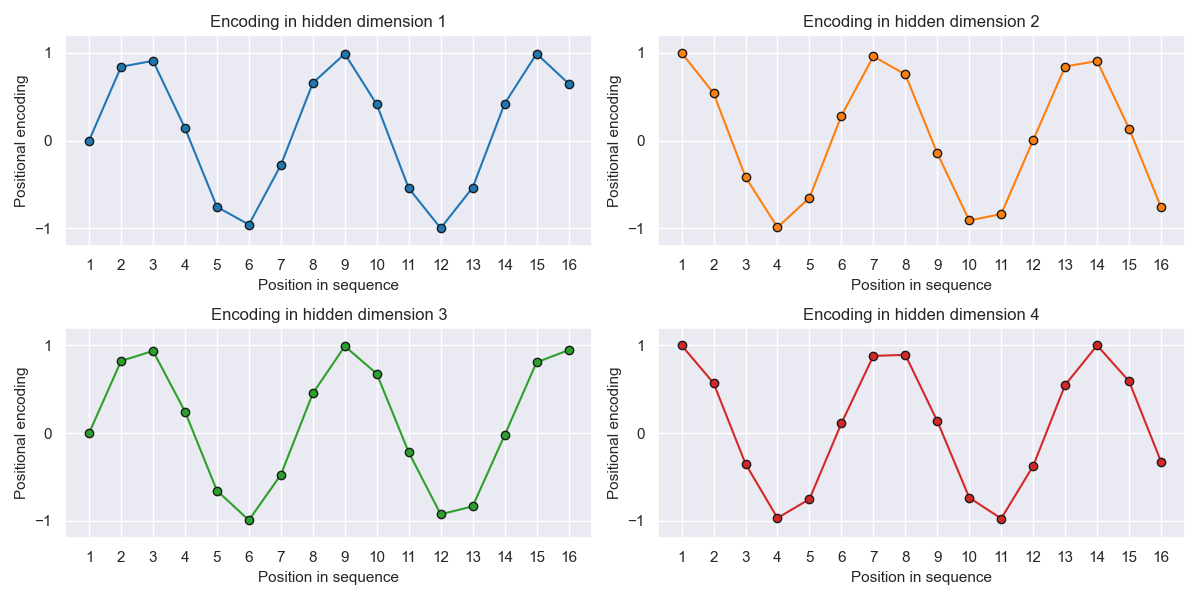
\includegraphics[width=1.0\textwidth]{Images/position_encoder.png}
    \vspace{0.3cm}
    \caption{Minh họa trực quan giá trị Positional Encoding trên 4 chiều ẩn đầu tiên. Các đường cong hình sin với tần số khác nhau giúp mô hình phân biệt vị trí trong chuỗi.}
    \label{fig:pos_encoding_vis}
\end{figure}

Hình \ref{fig:pos_encoding_vis} minh họa trực quan sự biến thiên giá trị của vector mã hóa vị trí trên bốn chiều ẩn đầu tiên đối với một chuỗi có độ dài $16$ bước. Các đồ thị cho thấy hàm lượng giác dao động trong khoảng từ $-1$ đến $1$ với tần số khác nhau tùy thuộc vào chỉ số của chiều không gian. Cụ thể, các chiều có chỉ số thấp thể hiện tần số dao động cao, trong khi các chiều cao hơn sở hữu bước sóng dài hơn. Cơ chế biến đổi tần số này kiến tạo nên một mẫu hình đặc trưng riêng biệt cho mỗi vị trí $pos$, hỗ trợ mô hình Transformer dễ dàng học được mối quan hệ vị trí tương đối giữa các token trong chuỗi.

\section{Biểu diễn Đa phương thức}
Trong kỷ nguyên dữ liệu lớn, thông tin về sản phẩm không còn bị giới hạn ở các mã định danh hay thuộc tính cấu trúc đơn giản, mà đã mở rộng sang các dạng dữ liệu phi cấu trúc phong phú như văn bản mô tả và hình ảnh minh họa. Học đa phương thức là phương pháp tiếp cận tiên tiến cho phép hệ thống tri nhận và thấu hiểu sâu sắc nội dung sản phẩm, từ đó xây dựng các vector biểu diễn embeddings giàu ngữ nghĩa. Cách tiếp cận này đặc biệt hiệu quả trong việc giải quyết bài toán cold-start đối với các sản phẩm mới chưa có lịch sử tương tác. Để khai thác hai luồng thông tin quan trọng nhất là ngôn ngữ và thị giác, đồ án áp dụng hai kiến trúc nền tảng đã chứng minh được hiệu quả vượt trội trong lĩnh vực này, lần lượt là BERT cho xử lý văn bản và ViT cho xử lý hình ảnh.

\subsection{Biểu diễn Văn bản: BERT}

Sự xuất hiện của mô hình BERT (Bidirectional Encoder Representations from Transformers)\cite{14} đã tạo ra một bước tiến quan trọng trong lĩnh vực xử lý ngôn ngữ tự nhiên, đặc biệt là ứng dụng trong việc trích xuất đặc trưng văn bản cho các hệ thống gợi ý hiện đại. Trước khi các mô hình ngôn ngữ lớn trở nên phổ biến, các phương pháp nhúng từ truyền thống như Word2Vec\cite{15} hay GloVe chủ yếu dựa trên cơ chế tạo ra các vector nhúng tĩnh. Hạn chế căn bản của cách tiếp cận này là việc gán một vector biểu diễn cố định duy nhất cho mỗi từ vựng, bất kể sự biến thiên về ngữ nghĩa trong các ngữ cảnh khác nhau.

Vấn đề này trở nên đặc biệt nghiêm trọng trong miền dữ liệu thương mại điện tử, nơi các từ khóa thường mang tính đa nghĩa cao. Điển hình như từ khóa "Chuột", ngữ nghĩa của nó thay đổi hoàn toàn khi xuất hiện trong cụm "Chuột máy tính Logitech" thuộc danh mục thiết bị điện tử so với cụm "Thuốc diệt chuột" thuộc danh mục hóa phẩm. Các mô hình tĩnh như Word2Vec không thể phân tách sự khác biệt này, dẫn đến sai lệch trong việc tính toán độ tương đồng sản phẩm. Ngược lại, BERT khắc phục triệt để nhược điểm trên thông qua cơ chế tạo ra các vector nhúng động, cho phép biểu diễn chính xác ngữ nghĩa của từ dựa trên sự phụ thuộc vào các từ lân cận trong câu.

Về mặt kiến trúc, BERT được xây dựng dựa trên sự chồng xếp của các lớp mã hóa trong kiến trúc Transformer. Khác biệt so với các mô hình tự hồi quy như GPT vốn chỉ xử lý thông tin đơn chiều từ trái sang phải, BERT áp dụng cơ chế Mô hình hóa ngôn ngữ che mặt nạ (Masked Language Modeling - MLM). Cơ chế này cho phép mô hình tiếp nhận và tổng hợp luồng thông tin ngữ cảnh hai chiều đồng thời, giúp nắm bắt cấu trúc cú pháp và ngữ nghĩa sâu sắc hơn. Như được minh họa chi tiết trong Hình \ref{fig:bert_architecture} \cite{14}, quy trình vận hành của BERT được chia thành hai giai đoạn kế tiếp nhau trên cùng một nền tảng kiến trúc thống nhất.
\begin{figure}[H]
    \centering
    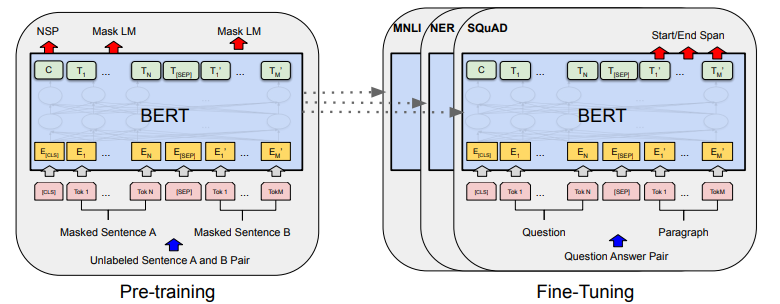
\includegraphics[width=0.9\textwidth]{Images/bert.png}
    \vspace{0.5cm}
    \caption{Quy trình Tiền huấn luyện và Tinh chỉnh của BERT.}
    \label{fig:bert_architecture}
\end{figure}

\noindent \textbf{Giai đoạn Tiền huấn luyện}

Giai đoạn tiền huấn luyện đóng vai trò nền tảng trong quy trình xây dựng mô hình, tại đó hệ thống tiếp thu các biểu diễn ngôn ngữ tổng quát thông qua việc khai thác khối lượng lớn dữ liệu văn bản thô chưa được gán nhãn. Quá trình học tập này vận hành dựa trên cơ chế tự giám sát, tập trung tối ưu hóa đồng thời hai tác vụ cốt lõi nhằm nắm bắt sâu sắc cấu trúc ngôn ngữ.

Đầu tiên là tác vụ Masked Language Modeling - MLM. Khác với phương pháp dự đoán từ tiếp theo theo tuần tự truyền thống, tác vụ này yêu cầu hệ thống phải khôi phục và tái tạo chính xác các đơn vị từ vựng đã bị che khuất ngẫu nhiên trong câu. Cơ chế này buộc mô hình phải tổng hợp và thấu hiểu ngữ cảnh hai chiều từ cả phía trước và phía sau của từ mục tiêu để đưa ra suy luận hợp lý nhất. Song song với đó là tác vụ dự đoán câu tiếp theo hay NSP, được thiết kế nhằm mục đích giúp mô hình thấu hiểu mối quan hệ logic và sự liên kết giữa các đoạn văn bản. Cụ thể, hệ thống học cách xác định xem một câu B bất kỳ có phải là câu nối tiếp thực tế về mặt ngữ nghĩa của câu A hay không, qua đó nắm bắt được cấu trúc diễn ngôn ở cấp độ cao hơn so với việc chỉ xử lý các từ ngữ riêng lẻ.

\noindent \textbf{Giai đoạn Tinh chỉnh}

Giai đoạn tinh chỉnh đóng vai trò là bước chuyển giao tri thức quan trọng, nơi mô hình áp dụng các biểu diễn ngôn ngữ tổng quát đã học được vào các tác vụ hạ nguồn cụ thể. Về mặt quy trình, thay vì khởi tạo ngẫu nhiên, mô hình kế thừa toàn bộ trọng số tham số từ giai đoạn tiền huấn luyện làm điểm bắt đầu, sau đó tiến hành tối ưu hóa tiếp tục trên các tập dữ liệu có gán nhãn chuyên biệt. Điểm mấu chốt là toàn bộ các tham số của mạng lưới đều được cập nhật đồng bộ trong quá trình này để thích nghi tốt nhất với đặc thù của từng bài toán riêng biệt. Trong phạm vi của hệ thống gợi ý, thay vì giải quyết các tác vụ ngôn ngữ tổng quát, quá trình tinh chỉnh được thiết kế chuyên biệt nhằm tối ưu hóa khả năng đọc hiểu tiêu đề và mô tả mặt hàng. Mục tiêu cuối cùng là trích xuất ra các vector đặc trưng văn bản chứa đựng trọn vẹn ngữ nghĩa sản phẩm, phục vụ trực tiếp cho việc xây dựng tháp sản phẩm.

Một đặc điểm kiến trúc nổi bật tạo nên sự thành công của BERT chính là tính nhất quán về cấu trúc. Hệ thống duy trì nguyên vẹn khối kiến trúc mã hóa Transformer đa tầng xuyên suốt quá trình huấn luyện sơ bộ và tinh chỉnh, đảm bảo luồng xử lý thông tin không bị gián đoạn. Sự thay đổi duy nhất chỉ diễn ra ở lớp đầu ra cuối cùng, nơi được thiết kế lại linh hoạt để tương thích với định dạng dự đoán của từng tác vụ đích, giúp mô hình đạt được hiệu suất cao mà không cần thay đổi đáng kể về mặt cấu trúc lõi.

Về cơ chế xử lý cốt lõi, thay vì sử dụng các mạng truy hồi truyền thống, BERT kế thừa trực tiếp sức mạnh từ kiến trúc Multi-Head Self-Attention đã được phân tích chi tiết tại Mục \ref{subsec:scaled_attention}. Điểm đột phá của mô hình nằm ở cách khai thác cơ chế sự chú ý này theo hướng hai chiều triệt để. Bằng việc tính toán trọng số thông qua các khối ma trận Truy vấn, Khóa và Giá trị, mỗi token trong câu đầu vào đều có khả năng quan sát và thu thập ngữ cảnh trực tiếp từ tất cả các token còn lại ở cả phía trước và phía sau nó cùng một lúc. 

Đồng thời, việc tận dụng kiến trúc chú ý đa đầu cho phép BERT tri giác thông tin văn bản từ nhiều không gian biểu diễn song song. Sự phân công nhiệm vụ tự động giữa các đầu chú ý, ví dụ một đầu chuyên bóc tách cấu trúc cú pháp trong khi đầu khác rà soát mối liên kết từ vựng tầm xa, giúp vector đầu ra của mô hình hội tụ đầy đủ các sắc thái ngôn ngữ. Nhờ sự kế thừa chặt chẽ này, BERT tạo ra các biểu diễn văn bản mang độ sâu ngữ nghĩa vượt trội, đáp ứng hoàn hảo yêu cầu khắt khe về việc thấu hiểu mô tả sản phẩm trong kiến trúc truy xuất đa phương thức.

Trong ngữ cảnh cụ thể của hệ thống gợi ý, mục tiêu đặt ra là thu được một vector đại diện duy nhất cho toàn bộ văn bản đầu vào. Để thực hiện điều này, BERT bổ sung một token đặc biệt ký hiệu là \texttt{[CLS]} vào vị trí đầu tiên của chuỗi. Sau khi đi qua toàn bộ các lớp mã hóa Transformer, vector đầu ra tương ứng với vị trí \texttt{[CLS]} này được coi là biểu diễn tổng hợp tinh túy nhất của cả câu:
\begin{equation}
    h_{\texttt{[CLS]}} = \text{BERT}(x_1, \dots, x_n)
\end{equation}
Vector $h_{\texttt{[CLS]}}$ này có khả năng nắm bắt được các đặc trưng ngữ nghĩa bậc cao như danh mục sản phẩm, tính năng nổi bật hay sắc thái cảm xúc trong bài đánh giá, mang lại hiệu quả vượt trội so với các phương pháp biểu diễn thô sơ như \textit{Bag-of-Words} truyền thống.

\subsection{Biểu diễn Hình ảnh: ViT}

Trong giai đoạn trước năm 2020, các kiến trúc mạng nơ-ron tích chập, viết tắt là CNN, với những đại diện tiêu biểu như ResNet hay EfficientNet được xem là chuẩn mực hàng đầu cho các tác vụ thị giác máy tính. Thành công này chủ yếu bắt nguồn từ khả năng khai thác hiệu quả các thiên kiến quy nạp về tính cục bộ và tính bất biến tịnh tiến đặc trưng của dữ liệu hình ảnh. Đối lập với bức tranh đó, kiến trúc Transformer\cite{12} lại đang khẳng định vị thế độc tôn và tạo ra những bước tiến vượt bậc trong lĩnh vực xử lý ngôn ngữ tự nhiên.

Bối cảnh công nghệ này đã thúc đẩy sự ra đời của Vision Transformer, hay còn gọi là ViT, nhằm giải quyết câu hỏi khoa học về tính khả thi của việc áp dụng trực tiếp kiến trúc Transformer thuần túy lên dữ liệu thị giác. Cách tiếp cận của ViT mang tính đột phá khi loại bỏ hoàn toàn sự phụ thuộc vào các lớp tích chập truyền thống để chuyển sang mô hình hóa bức ảnh dưới dạng một chuỗi các phần tử tuần tự, tương tự như cơ chế xử lý các đoạn văn bản.

Quyết định thay thế mạng tích chập truyền thống bằng kiến trúc Vision Transformer được củng cố bởi nghiên cứu mang tính đột phá của Dosovitskiy và cộng sự\cite{11}. Trong công trình này, nhóm tác giả đã chứng minh tính khả thi và hiệu quả vượt trội của việc áp dụng cơ chế tự chú ý trực tiếp lên dữ liệu hình ảnh quy mô lớn. Thay vì phụ thuộc vào các thiên kiến quy nạp về tính cục bộ như trong mạng ResNet hay EfficientNet, phương pháp này xử lý bức ảnh như một chuỗi các mảnh ghép độc lập, cho phép mô hình nắm bắt được các mối quan hệ ngữ nghĩa toàn cục giữa các vùng ảnh xa nhau ngay từ những lớp đầu tiên.

Rào cản kỹ thuật lớn nhất khi chuyển giao kiến trúc Transformer từ miền dữ liệu chuỗi sang dữ liệu hình ảnh nằm ở gánh nặng tính toán khổng lồ. Do cơ chế tự chú ý sở hữu độ phức tạp thuật toán bậc hai $\mathcal{O}(N^2)$ tỷ lệ thuận với số lượng phần tử đầu vào $N$, việc mô hình hóa trực tiếp từng điểm ảnh đơn lẻ như một đơn vị \textit{token} sẽ dẫn đến sự bùng nổ về chi phí tài nguyên. Đơn cử, một hình ảnh có kích thước tiêu chuẩn $224 \times 224$ sẽ tạo ra một chuỗi đầu vào lên tới 50.176 phần tử, khiến việc xây dựng ma trận chú ý trở nên bất khả thi đối với năng lực phần cứng hiện tại.

Mô hình Vision Transformer giải quyết triệt để vấn đề này thông qua kỹ thuật phân mảnh hay còn gọi là \textit{Patching}. Quy trình xử lý bắt đầu bằng việc chia nhỏ hình ảnh đầu vào $I \in \mathbb{R}^{H \times W \times C}$ thành một lưới các vùng cục bộ không chồng lấn có kích thước cố định $P \times P$, tạo ra tổng cộng $N = \frac{HW}{P^2}$ mảnh con. Tiếp theo, mỗi mảnh ảnh này được trải phẳng thành một vector một chiều và được đưa qua một phép chiếu tuyến tính có thể học được để ánh xạ vào không gian biểu diễn tiềm ẩn với số chiều $D$. Cuối cùng, nhằm mục đích khôi phục và bảo toàn thông tin về cấu trúc không gian vốn bị phá vỡ trong quá trình trải phẳng, các vector mã hóa vị trí $E_{\text{pos}}$ được cộng bổ sung trực tiếp vào các vector đặc trưng của từng mảnh trước khi đưa vào khối mã hóa Transformer. Quy trình xử lý chi tiết được mô tả trực quan thông qua Hình \ref{fig:vit_architecture} \cite{11}.

\begin{figure}[H]
    \centering
    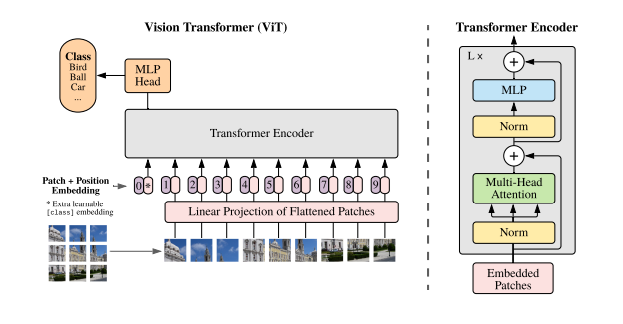
\includegraphics[width=0.9\textwidth]{Images/Vit.png}
    \vspace{0.5cm}
    \caption{Sơ đồ kiến trúc Vision Transformer.}
    \label{fig:vit_architecture}
\end{figure}

Bước tiếp theo là việc khởi tạo token phân loại. Một vector tham số có thể học được, thường được ký hiệu là token lớp, được chèn vào vị trí đầu tiên của chuỗi các vector mảnh ảnh. Token đặc biệt này đóng vai trò như một bộ thu nhận thông tin toàn cục; sau khi đi qua toàn bộ mạng nơ-ron, trạng thái đầu ra tại vị trí này sẽ được sử dụng làm đại diện tổng quát duy nhất cho toàn bộ bức ảnh, tương tự như cơ chế của token CLS trong mô hình ngôn ngữ BERT.

Chuỗi vector kết hợp này sau đó được đưa vào khối mã hóa Transformer Encoder, bao gồm nhiều lớp xử lý lặp lại liên tiếp. Trong mỗi lớp, cơ chế chú ý đa đầu đóng vai trò hạt nhân, cho phép mỗi mảnh ảnh có khả năng quan sát và liên kết ngữ nghĩa với tất cả các mảnh ảnh khác, bất kể khoảng cách không gian giữa chúng. Dữ liệu sau đó tiếp tục đi qua mạng nơ-ron truyền thẳng MLP để trích xuất các đặc trưng bậc cao. Để đảm bảo sự ổn định và khả năng hội tụ của quá trình huấn luyện sâu, kỹ thuật chuẩn hóa lớp Layer Normalization được áp dụng trước mỗi khối chức năng, kết hợp cùng các kết nối tắt nhằm duy trì dòng chảy thông tin và hạn chế hiện tượng triệt tiêu đạo hàm.

Cuối cùng, tại lớp đầu ra của khối mã hóa, chỉ duy nhất vector ứng với vị trí của token phân loại được trích xuất. Vector này mang trong mình thông tin ngữ nghĩa cô đọng nhất của bức ảnh và được đưa vào khối MLP Head để thực hiện các tác vụ đích như phân loại đối tượng hoặc tạo vector biểu diễn cho hệ thống gợi ý.\\

Sự khác biệt nền tảng định hình nên ưu thế của Vision Transformer so với mạng tích chập CNN nằm ở bản chất của trường tiếp nhận thông tin. Đối với các mạng tích chập truyền thống, trường tiếp nhận mang tính chất cục bộ nghiêm ngặt, nghĩa là các lớp tích chập khởi đầu chỉ có khả năng ghi nhận và xử lý tín hiệu từ các điểm ảnh lân cận. Sự tổng hợp thông tin toàn cục chỉ có thể đạt được một cách gián tiếp và thụ động thông qua quá trình chồng xếp nhiều lớp mạng sâu nhằm mở rộng dần vùng quan sát. Ngược lại, Vision Transformer tận dụng sức mạnh của cơ chế tự chú ý để phá vỡ giới hạn không gian này. Ngay từ lớp xử lý đầu tiên, mỗi mảnh ảnh đã thiết lập được sự tương tác trực tiếp với tất cả các mảnh ảnh khác, cho phép mô hình có cái nhìn toàn cảnh tức thời về đối tượng.

Đặc tính kỹ thuật này mang lại ý nghĩa quan trọng trong ngữ cảnh của bài toán gợi ý sản phẩm, đặc biệt đối với các ngành hàng đề cao tính thẩm mỹ như thời trang hay nội thất. Trong những lĩnh vực này, vẻ đẹp và giá trị của sản phẩm thường không chỉ nằm ở các chi tiết riêng lẻ mà phụ thuộc vào bố cục tổng thể cùng sự phối hợp giữa các thành phần nằm cách xa nhau, chẳng hạn như sự tương thích giữa cổ áo và gấu váy hay sự đồng điệu giữa màu sắc giày và họa tiết thương hiệu. Năng lực thấu hiểu các mối quan hệ ngữ nghĩa toàn cục và phức tạp này cho phép Vision Transformer trích xuất được các vector đặc trưng giàu thông tin hơn, mang lại hiệu quả vượt trội cho tác vụ gợi ý so với các phương pháp tích chập truyền thống.

\subsection{Cơ chế Hợp nhất Không gian Vector}
\label{sec:attention_theory}

Một sản phẩm trên thực tế có thể có nhiều hình thức biểu diễn như văn bản, hình ảnh, video. Nghiên cứu của Radford \cite{16} đã khẳng định tầm quan trọng của việc khai thác đa phương thức để hiểu sâu ngữ nghĩa đối tượng. Tuy nhiên, thay vì chỉ so khớp đơn thuần, việc hợp nhất các đặc trưng này thành một biểu diễn duy nhất là yêu cầu bắt buộc đối với tháp sản phẩm trong kiến trúc Two-Tower. Hình \ref{fig:fusion_architecture} \cite{16} mô tả kiến trúc hợp nhất được đề xuất.
\begin{figure}[H]
    \centering
    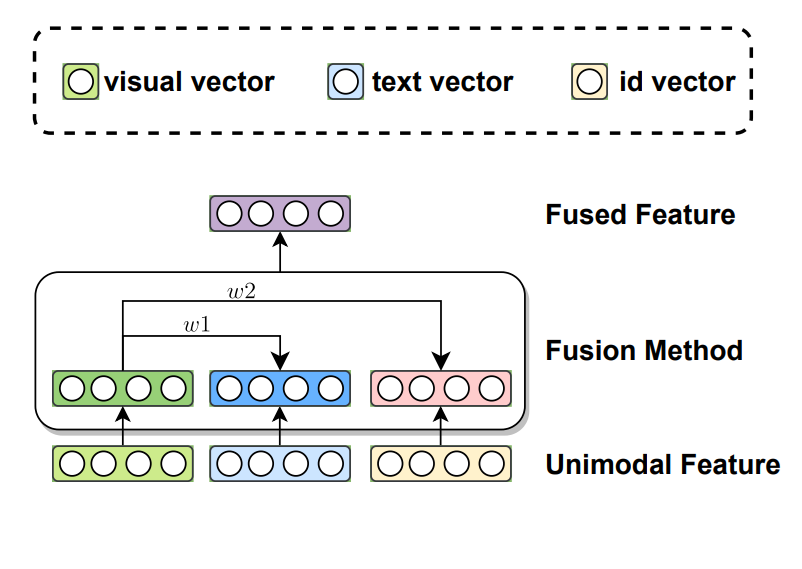
\includegraphics[width=0.9\textwidth]{Images/fusion.png}
    \vspace{0.5cm}
    \caption{Sơ đồ kiến trúc Multi-Modality Fusion.}
    \label{fig:fusion_architecture}
\end{figure}

Hạn chế căn bản của các phương pháp hợp nhất truyền thống như phép nối vector hay phép cộng trung bình nằm ở giả định cứng nhắc rằng mức độ quan trọng của hình ảnh và văn bản là tương đương nhau đối với mọi sản phẩm. Trong thực tế dữ liệu thương mại điện tử luôn tồn tại sự bất cân xứng về chất lượng thông tin khi một số mặt hàng sở hữu hình ảnh trực quan sắc nét nhưng phần mô tả lại sơ sài hoặc ngược lại. Để giải quyết vấn đề này đồ án áp dụng cơ chế Hợp nhất có cổng hay còn gọi là Gated Fusion được phát triển dựa trên nền tảng lý thuyết mạng nơ-ron đa phương thức của Arevalo và cộng sự\cite{24}.

Quy trình xử lý dữ liệu để tạo ra vector đại diện sản phẩm được thực hiện qua ba giai đoạn tuần tự, đảm bảo tính đồng bộ về mặt toán học giữa các luồng dữ liệu khác biệt.

Đầu tiên là giai đoạn đồng bộ hóa không gian biểu diễn. Xuất phát từ thực tế rằng đầu ra từ các bộ mã hóa hình ảnh và văn bản (như ViT cho ảnh và BERT cho văn bản) thường sở hữu số chiều khác nhau và nằm trong các phân phối đặc trưng riêng biệt, hệ thống cần áp dụng phép chiếu tuyến tính để dung hòa sự khác biệt này. Cụ thể, hai ma trận trọng số $\mathbf{W}_v$ và $\mathbf{W}_t$ được sử dụng để ánh xạ các đặc trưng thô về cùng một không gian vector tiềm ẩn có kích thước cố định $d$, tạo tiền đề cho sự tương tác trực tiếp:
\begin{align}
    \mathbf{v}_I &= \tanh(\mathbf{W}_v \cdot I_{\text{raw}} + \mathbf{b}_v) \\
    \mathbf{v}_T &= \tanh(\mathbf{W}_t \cdot T_{\text{raw}} + \mathbf{b}_t)
\end{align}
Tiếp theo, các vector đặc trưng sau khi đồng bộ được đưa vào cơ chế Hợp nhất có cổng (\textit{Gated Mechanism}). Đây là thành phần cốt lõi của mô hình, đóng vai trò như một van điều tiết thông minh nhằm xác định mức độ quan trọng của từng luồng thông tin. Một giá trị cổng kiểm soát $z$ được tính toán dựa trên sự kết hợp của cả hai loại dữ liệu, sử dụng hàm kích hoạt Sigmoid $\sigma$ để nén giá trị về khoảng $(0, 1)$:
\begin{equation}
    z = \sigma(\mathbf{W}_z \cdot [\mathbf{v}_I, \mathbf{v}_T] + \mathbf{b}_z)
\end{equation}
Dựa trên giá trị cổng này, vector hợp nhất $\mathbf{v}_{\text{fusion}}$ được xác định bằng tổ hợp tuyến tính có trọng số. Cơ chế này cho phép mô hình linh hoạt chuyển đổi sự tập trung; khi $z$ tiệm cận $1$, hệ thống sẽ ưu tiên khai thác tín hiệu thị giác và ngược lại sẽ dựa nhiều vào văn bản khi $z$ tiến về $0$:
\begin{equation}
    \mathbf{v}_{\text{fusion}} = z \odot \mathbf{v}_I + (1 - z) \odot \mathbf{v}_T
\end{equation}

Cuối cùng, để hoàn thiện biểu diễn của sản phẩm, vector hợp nhất $\mathbf{v}_{\text{fusion}}$ trải qua bước chuẩn hóa theo chuẩn $L_2$ nhằm tạo ra vector đầu ra $\mathbf{v}_{\text{item}}$:
\begin{equation}
    \mathbf{v}_{\text{item}} = \frac{\mathbf{v}_{\text{fusion}}}{\|\mathbf{v}_{\text{fusion}}\|_2}
\end{equation}
Bước xử lý này đảm bảo độ dài của mọi vector đại diện đều bằng $1$. Về mặt hình học, điều này giúp phép nhân vô hướng với vector người dùng ở giai đoạn truy xuất sau này trở thành thước đo độ tương đồng Cosine chuẩn xác, đồng thời góp phần ổn định đáng kể quá trình huấn luyện của mạng nơ-ron.

\section{Nắm bắt chuỗi hành vi trong ResSys}

\subsection{Sự tiến hóa của các Hệ thống Gợi ý Tuần tự: Từ Markov đến RNN}

Trong bối cảnh thương mại điện tử, sở thích của người dùng là một quá trình động, thay đổi liên tục theo thời gian và chịu ảnh hưởng mạnh mẽ bởi ngữ cảnh ngắn hạn. Trước khi kỷ nguyên học sâu bùng nổ, Chuỗi Markov đóng vai trò là nền tảng lý thuyết chủ đạo. Mô hình này, tiêu biểu như FPMC \cite{26}, xem lịch sử người dùng là các trạng thái chuyển đổi và đưa ra giả định theo tính chất Markov bậc một: hành động tiếp theo chỉ phụ thuộc duy nhất vào hành động ngay trước đó. Dù hiệu quả trong việc nắm bắt tương tác ngắn hạn giữa các cặp sản phẩm liền kề, Chuỗi Markov lại tỏ ra yếu kém trong việc ghi nhớ các chuỗi hành vi dài.

Để giải quyết bài toán phụ thuộc xa, Mạng nơ-ron tái phát RNN và các biến thể như GRU, LSTM đã được áp dụng. Điển hình là kiến trúc GRU4Rec \cite{30}, cho phép mô hình hóa toàn bộ lịch sử hành vi thành một chuỗi liên tục thông qua cơ chế cập nhật trạng thái ẩn, qua đó trích xuất được sở thích dài hạn của người dùng. Mặc dù vượt trội hơn Markov, kiến trúc RNN vẫn tồn tại những nhược điểm chí mạng: bản chất tính toán tuần tự khiến quá trình huấn luyện không thể song song hóa trên các phần cứng hiện đại như GPU, đồng thời hiện tượng triệt tiêu đạo hàm vẫn xảy ra với các chuỗi quá dài. Những rào cản phần cứng và thuật toán này chính là động lực thúc đẩy sự chuyển dịch công nghệ sang các kiến trúc dựa trên cơ chế Tự chú ý trong giai đoạn sau này.

\subsection{Kiến trúc SASRec}

Dựa trên sự thành công vang dội của cơ chế Attention trong xử lý ngôn ngữ tự nhiên, Kang và McAuley (2018) \cite{7} đã đề xuất mô hình SASRec. Đây là kiến trúc được đồ án lựa chọn làm nòng cốt cho Tháp Người dùng. SASRec thay thế hoàn toàn các lớp hồi quy bằng cơ chế Tự chú ý (Self-Attention), cho phép mô hình xác định trọng số quan trọng của từng sản phẩm trong quá khứ đối với sản phẩm mục tiêu dựa trên mối quan hệ ngữ nghĩa thay vì khoảng cách vị trí cố định. Nội dung trong mục này nói về mô hình SASRec của Kang và McAuley \cite{7}.

Mô hình SASRec vận hành thông qua một chuỗi các tầng xử lý tuần tự, khởi đầu với Tầng Nhúng. Kế thừa trực tiếp nguyên lý đã được phân tích tại Mục \ref{subsec:positional_encoding} về giới hạn nhận thức thứ tự của mạng Transformer, hệ thống bắt buộc phải tích hợp thông tin vị trí vào chuỗi đầu vào. Cụ thể, mô hình thực hiện phép cộng trực tiếp ma trận biểu diễn đặc trưng của sản phẩm $M$ với một ma trận vị trí có thể học được $P$, tạo thành một không gian biểu diễn tổng hợp $\hat{E} = M + P$.

Ngay sau bước chuẩn bị dữ liệu, ma trận tổng hợp này được truyền thẳng vào khối mạng Self-Attention. Dựa trên nền tảng toán học của cơ chế sự chú ý đã được định nghĩa chi tiết tại Mục \ref{subsec:scaled_attention}, SASRec tiến hành điều chỉnh kỹ thuật để tương thích tuyệt đối với bài toán chuỗi thời gian. Cụ thể, mô hình tích hợp thêm cơ chế che chắn nhân quả nhằm giới hạn tầm nhìn của mạng nơ-ron. Cơ chế này ép buộc các đầu chú ý chỉ được phép quét và tính toán mức độ tương quan đối với các sản phẩm mà người dùng đã tương tác trong quá khứ, triệt tiêu hoàn toàn hiện tượng rò rỉ thông tin từ tương lai. Nhờ sự kết hợp này, SASRec có khả năng nắm bắt chính xác dòng chảy biến thiên trong sở thích mua sắm của khách hàng ở từng thời điểm cụ thể. Một yếu tố kỹ thuật then chốt tại đây là việc áp dụng Mặt nạ nhân quả (\textit{Causal Masking}). Cơ chế này đảm bảo rằng khi dự đoán tại thời điểm $t$, mô hình chỉ được phép tiếp cận thông tin từ thời điểm $1$ đến $t$, ngăn chặn tuyệt đối việc rò rỉ thông tin từ tương lai và bảo toàn tính nhân quả của dữ liệu chuỗi.

Để khai thác các đặc trưng sâu hơn sau lớp Attention, mô hình tích hợp Mạng truyền thẳng từng điểm (\textit{Point-wise Feed-Forward Network}). Mạng này thực hiện các phép biến đổi phi tuyến cho từng vị trí một cách độc lập nhưng chia sẻ chung bộ trọng số, giúp mô hình nắm bắt các tương tác phức tạp giữa các chiều ẩn. Kiến trúc tổng thể của SASRec được hình thành bằng cách xếp chồng $b$ khối xử lý như vậy nhằm giải quyết vấn đề quá khớp và mất ổn định khi huấn luyện mạng sâu, nhóm tác giả áp dụng cấu trúc tương tự Transformer bao gồm Chuẩn hóa lớp (\textit{Layer Normalization}) để ổn định phân phối, Dropout để điều hòa quá trình học, và Kết nối tắt (\textit{Residual Connections}) để hỗ trợ lan truyền thông tin. Toàn bộ quy trình này được mô hình hóa qua công thức tổng quát cho mỗi lớp con $g$:
\begin{equation}
    g(x) = x + \text{Dropout}(g(\text{LayerNorm}(x)))
\end{equation}
như được mô tả trong tài liệu của Kang và McAuley.

Tại Tầng Dự đoán cuối cùng, sau khi đi qua $b$ khối xử lý, vector đại diện $\mathbf{F}_t^{(b)}$ tại bước $t$ sẽ được sử dụng để dự đoán sản phẩm tiếp theo. Điểm số tương quan $r_{i,t}$ được xác định bằng tích vô hướng giữa vector đại diện này và vector nhúng của sản phẩm mục tiêu $\mathbf{N}_i$. Để tối ưu hóa kích thước mô hình và hạn chế quá khớp, SASRec áp dụng chiến lược Shared Item Embedding, tức là sử dụng chung một ma trận nhúng cho cả đầu vào và đầu ra ($\mathbf{N}=\mathbf{M}$). Các tác giả lập luận rằng tính phi tuyến mạnh mẽ của mạng truyền thẳng là đủ để mô hình giải quyết vấn đề bất đối xứng (mua điện thoại thì có thể đề xuất ốp lưng nhưng mua ốp lưng thì không đề xuất điện thoại) trong các chuyển đổi hành vi mua sắm mà không cần thiết phải tách biệt hai ma trận này.

Dựa trên các kết quả thực nghiệm được công bố bởi Kang và McAuley, mô hình SASRec đã chứng minh được hiệu năng vượt trội so với các kiến trúc tiền nhiệm như GRU4Rec hay Caser nhờ vào hai ưu thế kỹ thuật then chốt.

Đầu tiên là khả năng nắm bắt các phụ thuộc dài hạn trong chuỗi hành vi. Đối với các mạng hồi quy truyền thống, thông tin buộc phải lan truyền tuần tự qua từng bước thời gian, tạo ra độ dài đường dẫn tỷ lệ thuận với độ dài chuỗi $\mathcal{O}(n)$. Ngược lại, cơ chế Tự chú ý cho phép thiết lập kết nối trực tiếp giữa hai sản phẩm bất kỳ bất kể khoảng cách vị trí. Đặc tính này rút ngắn độ dài đường truyền tín hiệu xuống mức hằng số $\mathcal{O}(1)$, giúp mô hình duy trì và truy xuất hiệu quả các sở thích người dùng đã hình thành từ quá khứ xa mà không bị suy hao thông tin.

Ưu điểm thứ hai nằm ở hiệu suất tính toán và khả năng mở rộng. Khác với tính chất tuần tự bắt buộc của mạng hồi quy khiến quá trình xử lý không thể tận dụng triệt để sức mạnh của GPU, các phép toán ma trận trong SASRec có thể được thực thi song song trên toàn bộ chiều dài chuỗi. Sự cải tiến này mang lại lợi ích to lớn về mặt tốc độ; các thử nghiệm cho thấy thời gian huấn luyện của SASRec nhanh hơn gấp mười lần so với các mô hình dựa trên mạng hồi quy hoặc tích chập, cho phép hệ thống dễ dàng mở rộng để xử lý các tập dữ liệu quy mô lớn.

\subsection{Kiến trúc Two tower cho Truy xuất Ứng viên}

\noindent \textbf{Bối cảnh và Vấn đề Quy mô}

Trong các hệ sinh thái thương mại điện tử quy mô lớn, thách thức kỹ thuật trọng yếu luôn nằm ở giai đoạn truy xuất (Retrieval). Tại đây, hệ thống buộc phải sàng lọc ra hàng trăm ứng viên tiềm năng từ một không gian dữ liệu khổng lồ chứa hàng triệu mặt hàng, với yêu cầu khắt khe về độ trễ tối thiểu, thường phải dưới 100 mili giây.

Trước bài toán này, các phương pháp truyền thống như Phân rã ma trận đã bộc lộ giới hạn do không thể nắm bắt các tương tác phi tuyến tính phức tạp. Quan trọng hơn, ngay cả các mô hình học sâu hiện đại như kiến trúc SASRec nguyên bản \cite{7} cũng vấp phải rào cản lớn khi triển khai thực tế. Do thiết kế theo hướng dự đoán đầu cuối (end-to-end classification) với chiến lược Shared Item Embedding, SASRec gốc trói buộc quá trình nội suy chuỗi hành vi của người dùng với ma trận định danh của toàn bộ sản phẩm vào cùng một đồ thị tính toán. Cấu trúc đóng gói này dẫn đến hai hệ lụy: thứ nhất, nó cản trở việc tích hợp các đặc trưng đa phương thức (văn bản, hình ảnh) để giải quyết bài toán cold-start; thứ hai, nó khiến việc quét và chấm điểm toàn bộ danh mục hàng triệu sản phẩm trong thời gian thực trở thành một gánh nặng tính toán bất khả thi.

Để giải quyết bài toán này, kiến trúc Mạng nơ-ron Hai tháp, hay còn được biết đến với tên gọi Bi-Encoder, đã trở thành chuẩn mực công nghiệp hiện đại. Mô hình này được tiên phong ứng dụng bởi YouTube \cite{9} và sau đó được tối ưu hóa hoàn thiện bởi Google \cite{8} cho các tác vụ xếp hạng quy mô lớn.

\vspace{0.3cm}

\noindent \textbf{Cấu trúc Mạng nơ-ron Hai tháp}

Về mặt bản chất, kiến trúc Hai tháp hoạt động dựa trên nguyên lý tách biệt quá trình mã hóa thành hai luồng xử lý độc lập nhằm tối ưu hóa tốc độ truy vấn. Cụ thể, hệ thống bao gồm Tháp Người dùng được ký hiệu là bộ mã hóa $f_\theta$, chịu trách nhiệm tổng hợp hồ sơ cá nhân và lịch sử hành vi để tạo ra vector biểu diễn người dùng $\mathbf{u}$ thuộc không gian $\mathbb{R}^d$. Song song với đó, Tháp Sản phẩm với bộ mã hóa $g_\phi$ tập trung khai thác các đặc trưng nội tại của vật phẩm để xây dựng vector biểu diễn tương ứng $\mathbf{v}$.

Điểm đặc trưng cốt lõi phân biệt thiết kế này với các mô hình khác là cơ chế tương tác muộn. Hai mạng nơ-ron hoàn toàn không chia sẻ thông tin hay tham số trong suốt quá trình trích xuất đặc trưng, mà chỉ thực hiện so khớp ở lớp cuối cùng. Tại đây, độ tương đồng hay mức độ phù hợp giữa người dùng và sản phẩm được ước lượng thông qua phép tính tích vô hướng đơn giản \cite{7}:
\begin{equation}
    s(x,y) = \langle u(x, \theta), v(y, \theta) \rangle
\end{equation}
Trong đó, $u(x, \theta)$ là hàm ánh xạ đặc trưng người dùng $x$, và $v(y, \theta)$ là hàm ánh xạ đặc trưng sản phẩm $y$ dựa trên bộ tham số mô hình $\theta$.

Cơ chế này cho phép hệ thống tính toán trước và lập chỉ mục các vector sản phẩm, giúp giảm đáng kể chi phí tính toán trực tuyến trong giai đoạn truy xuất thời gian thực.

\vspace{0.3cm}

\noindent \textbf{Chiến lược Huấn luyện: Học Tương phản}

Trong các kiến trúc Two-Tower hiện đại, chiến lược huấn luyện đã có sự chuyển dịch từ bài toán phân loại nhị phân truyền thống sang khuôn khổ Học tương phản (Contrastive Learning). Thách thức lớn nhất đối với các hệ thống truy xuất quy mô lớn nằm ở hàm mục tiêu: việc tính toán hàm Softmax trên toàn bộ không gian ứng viên (có thể lên tới hàng triệu sản phẩm) để xác định mẫu âm là bất khả thi về mặt tài nguyên tính toán và độ trễ. Để giải quyết vấn đề này, đồ án áp dụng giải pháp được đề xuất bởi Yi và cộng sự (2019) \cite{8}, sử dụng hàm mất mát Sampled Softmax kết hợp với kỹ thuật lấy mẫu âm trong lô.

Kỹ thuật này hoạt động dựa trên giả định thống kê rằng trong một lô dữ liệu ngẫu nhiên, các cặp người dùng và sản phẩm không tương ứng có xác suất rất cao là không liên quan đến nhau. Thay vì tiêu tốn chi phí để truy xuất và đào (mine) các mẫu âm từ kho dữ liệu bên ngoài, hệ thống tận dụng chính các sản phẩm của người dùng khác trong cùng một lô để làm mẫu âm.

Cụ thể, xét một lô dữ liệu có kích thước $B$. Với mỗi cặp mẫu dương $(\mathbf{u}_i, \mathbf{v}_i)$ (tương ứng với người dùng $i$ và sản phẩm thực tế $i$):
\begin{itemize}
    \item \textbf{Mẫu dương:} Là chính vector sản phẩm $\mathbf{v}_i$. Mục tiêu của mô hình là tối đa hóa độ tương đồng $s(\mathbf{u}_i, \mathbf{v}_i)$.
    \item \textbf{Mẫu âm:} Là tập hợp toàn bộ các vector sản phẩm $\mathbf{v}_j$ (với $j \neq i$) thuộc về các mẫu dữ liệu khác trong cùng batch đó. Như vậy, mỗi người dùng sẽ được so sánh với $1$ mẫu dương và $(B-1)$ mẫu âm nhân tạo này.
\end{itemize}

Để tối ưu hóa quá trình học biểu diễn vector, hệ thống sử dụng hàm mất mát InfoNCE (\ref{eq:infoNCE}). Hàm này có nhiệm vụ tối đa hóa xác suất dự đoán đúng sản phẩm mục tiêu $\mathbf{v}_i$ trong khi giảm thiểu xác suất của tập hợp $B-1$ sản phẩm nhiễu.

Phương pháp này không chỉ giải quyết triệt để bài toán hiệu năng tính toán mà còn được chứng minh là giúp mô hình học được các không gian biểu diễn phân tách tốt hơn, nhờ vào sự đa dạng và ngẫu nhiên của các mẫu âm được cập nhật liên tục trong mỗi bước huấn luyện.

\vspace{0.3cm}

\noindent \textbf{Ưu điểm về Triển khai Thực tế}

Lý do kiến trúc Two-Tower trở thành chuẩn mực thống trị trong bài toán Truy xuất bắt nguồn từ khả năng tách biệt hoàn toàn quá trình tính toán giữa hai thực thể người dùng và sản phẩm. Đặc tính kỹ thuật này cho phép tối ưu hóa quy trình xử lý thông qua hai giai đoạn riêng biệt. Trong giai đoạn ngoại tuyến (offline), nhờ sự độc lập của Tháp Sản phẩm, hệ thống có thể thực hiện tính toán trước vector biểu diễn cho toàn bộ không gian hàng hóa—có thể lên tới hàng triệu phần tử—và lưu trữ chúng dưới dạng chỉ mục tối ưu trong các cơ sở dữ liệu vector chuyên dụng như Milvus hay Faiss.

Chiến lược này tạo tiền đề cho hiệu suất vượt trội trong giai đoạn phục vụ trực tuyến (online serving). Khi nhận yêu cầu, hệ thống chỉ cần thực thi suy luận một lần duy nhất tại Tháp Người dùng để tạo ra vector truy vấn. Sau đó, thay vì phải quét toàn bộ cơ sở dữ liệu, việc xác định Top-K ứng viên tiềm năng được thực hiện thông qua các thuật toán ANN. Cơ chế này cho phép hệ thống duy trì độ trễ phản hồi ở mức dưới mili-giây, đồng thời đảm bảo tốc độ truy xuất không bị suy giảm tuyến tính khi quy mô kho hàng tăng lên, giải quyết triệt để bài toán về khả năng mở rộng của các hệ thống gợi ý hiện đại \cite{9}.

\section{Mô hình xếp hạng lại Reranking}
Sau khi giai đoạn Retrieval hoàn thành nhiệm vụ thu hẹp không gian tìm kiếm từ hàng triệu sản phẩm xuống một tập hợp ứng viên giới hạn, hệ thống đòi hỏi một cơ chế tinh vi hơn để phân tích chính xác mức độ phù hợp của từng ứng viên đối với nhu cầu của người dùng. Giai đoạn Reranking đảm nhận vai trò định chuẩn này. Việc chỉ sắp xếp lại vài chục đến vài trăm kết quả cho phép hệ thống triển khai các mô hình ngôn ngữ có độ phức tạp tính toán cao, mà điển hình và mạnh mẽ nhất hiện nay là kiến trúc Cross-Encoder.

\subsection{Lý thuyết Cross Encoder}

Mô hình Cross-Encoder là một kiến trúc mạng nơ-ron học sâu được xây dựng trực tiếp trên nền tảng của khối mã hóa (Encoder) thuộc mô hình Transformer, do Vaswani và cộng sự đề xuất vào năm 2017 \cite{49}. Sự trỗi dậy mạnh mẽ của Cross-Encoder trong lĩnh vực xếp hạng thông tin bắt đầu từ khi Nogueira và Cho (2019) ứng dụng thành công kiến trúc BERT vào bài toán đánh giá mức độ liên quan của văn bản \cite{50}. Nguyên lý hoạt động cốt lõi của Cross-Encoder nằm ở cách nó xử lý dữ liệu đầu vào và khai thác cơ chế tự chú ý.

\begin{figure}[H]
    \centering
    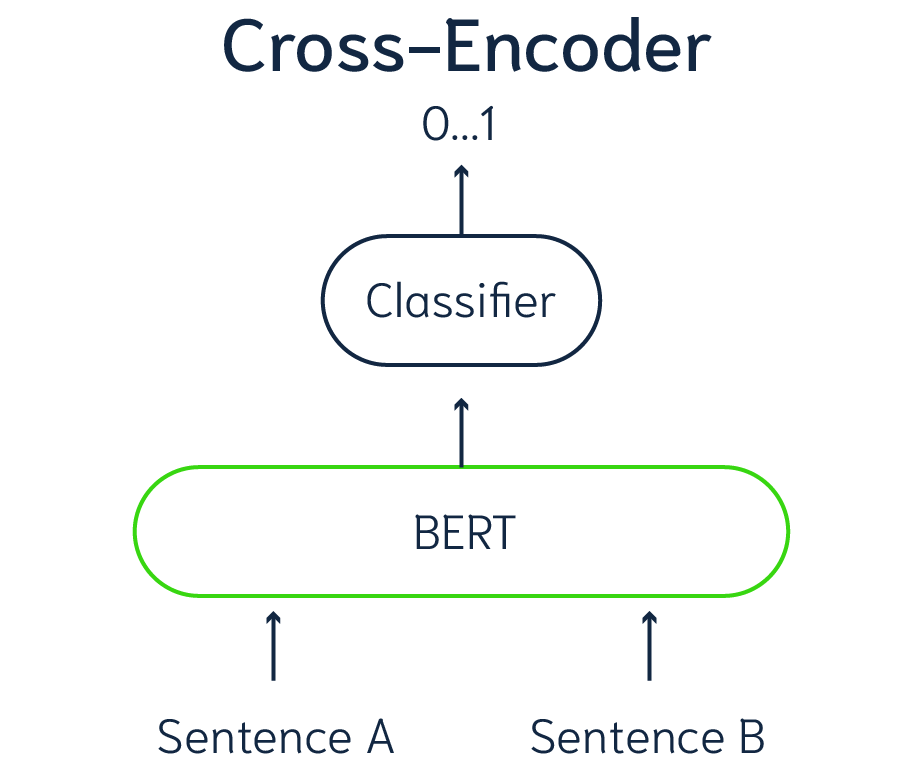
\includegraphics[width=0.5\textwidth]{Images/cross-encoder.png}
    \vspace{1em}
    \caption{Kiến trúc tổng quan của mô hình Cross-Encoder}
    \label{fig:cross_encoder_arch}
    
\end{figure}

Thay vì mã hóa độc lập từng đối tượng, Cross-Encoder yêu cầu ghép nối trực tiếp câu truy vấn ($Query$) và thông tin sản phẩm ($Item$) thành một chuỗi duy nhất trước khi đưa vào mô hình. Chuỗi đầu vào này thường được định dạng bằng các token đặc biệt, ví dụ như [CLS] Query [SEP] Item [SEP]. Ngay từ những lớp đầu tiên của mạng Transformer, cơ chế Tương tác sớm đã được kích hoạt. Thông qua ma trận Self-Attention, mỗi một từ khóa trong câu truy vấn đều có khả năng quan sát, tính toán trọng số và tương tác trực tiếp với toàn bộ các từ khóa nằm trong phần mô tả sản phẩm, và ngược lại. Quá trình này được lặp đi lặp lại qua nhiều tầng nơ-ron, giúp hệ thống không chỉ đối khớp từ khóa một cách máy móc mà còn thấu hiểu được ngữ cảnh, cấu trúc cú pháp và các hàm ý liên kết phức tạp.

Kết quả của toàn bộ quá trình tương tác chéo này được hội tụ vào token đặc biệt [CLS] ở tầng biểu diễn cuối cùng. Vector biểu diễn của token này mang theo toàn bộ thông tin tổng hợp về mối quan hệ ngữ nghĩa giữa $Query$ và $Item$. Cuối cùng, vector này được đưa qua một mạng nơ-ron truyền thẳng (Feed-Forward Network) kết hợp với hàm kích hoạt để chiếu thành một giá trị vô hướng duy nhất. Giá trị này đại diện cho điểm số xếp hạng, phản ánh chính xác mức độ liên quan của sản phẩm đối với mục tiêu tìm kiếm của người dùng.

\subsection{So sánh Cross Encoder và Bi Encoder}

Để hiểu rõ lý do tại sao kiến trúc hệ thống hiện đại bắt buộc phải duy trì hai giai đoạn với hai mô hình khác biệt, cần phải phân tích sự tương phản sâu sắc về cơ chế hoạt động cũng như sự đánh đổi giữa Cross-Encoder và Bi-Encoder. Nghiên cứu của Reimers và Gurevych (2019) về Sentence-BERT đã chỉ ra một cách hệ thống những ranh giới kỹ thuật này \cite{51}.

\begin{figure}[H]
    \centering
    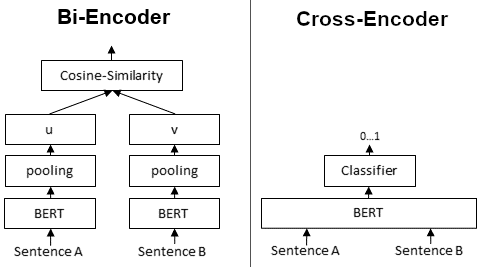
\includegraphics[width=1\textwidth]{Images/Bi_vs_Cross-Encoder.png}
    \vspace{1em}
    \caption{So sánh sự khác biệt giữa kiến trúc Bi-Encoder và Cross-Encoder}
    \label{fig:bi_vs_cross_comparison}
\end{figure}

Bi-Encoder, kiến trúc chủ đạo của giai đoạn Truy xuất, hoạt động dựa trên cơ chế Tương tác muộn. Nó sử dụng hai mạng Transformer độc lập để mã hóa câu truy vấn và sản phẩm thành hai vector dày đặc riêng biệt trong cùng một không gian học thuật. Sự so sánh chỉ diễn ra ở bước cuối cùng thông qua các phép tính đơn giản như độ tương đồng Cosine. Lợi thế tuyệt đối của Bi-Encoder là khả năng tính toán trước. Mọi sản phẩm trong kho đều được chuyển thành vector và lập chỉ mục từ trước, do đó khi có truy vấn, hệ thống chỉ mất vài mili giây để tìm ra các láng giềng gần nhất. Tuy nhiên, cái giá phải trả cho tốc độ là sự suy giảm về khả năng biểu diễn ngữ nghĩa. Việc nén toàn bộ ý nghĩa của một văn bản dài vào một vector có kích thước cố định gây ra hiện tượng thắt cổ chai thông tin. Mô hình mất đi khả năng đối khớp chính xác ở cấp độ từ vựng, dễ dẫn đến sai lệch khi người dùng tìm kiếm các sản phẩm có sự khác biệt rất nhỏ về từ ngữ nhưng khác biệt lớn về bản chất.

Ngược lại, Cross-Encoder khắc phục hoàn toàn nhược điểm này bằng cơ chế Tương tác sớm. Bằng cách cho phép các luồng thông tin giao thoa ngay từ đầu, nó duy trì được bức tranh toàn cảnh về mặt từ vựng và ngữ pháp. Ví dụ, trong ngữ cảnh thương mại điện tử, truy vấn "ốp lưng iPhone 15" và sản phẩm "iPhone 15 màu đen tặng kèm ốp lưng" có thể bị Bi-Encoder đánh giá là rất giống nhau vì không gian vector chứa nhiều từ khóa tương đồng. Tuy nhiên, Cross-Encoder với sự chú ý sâu sắc sẽ nhận ra vai trò chủ thể của cụm "ốp lưng" trong truy vấn không khớp với vai trò phụ trợ của nó trong tên sản phẩm, từ đó cho điểm xếp hạng thấp hơn.

Mặc dù có độ chính xác vượt trội, Cross-Encoder lại gặp phải rào cản chí mạng về khối lượng tính toán. Vì câu truy vấn và sản phẩm phải được ghép nối để tính toán lại từ đầu, độ phức tạp của cơ chế Self-Attention tăng lên theo bình phương độ dài chuỗi đầu vào. Việc áp dụng Cross-Encoder để so sánh một truy vấn với hàng triệu sản phẩm sẽ tiêu tốn một lượng tài nguyên và thời gian khổng lồ, vượt ra ngoài khả năng đáp ứng thời gian thực.

Chính sự bù trừ này đã định hình nên kiến trúc gợi ý đa giai đoạn. Bi-Encoder đóng vai trò như hệ thống lọc nhanh nhẹn, chấp nhận độ sai số nhất định để mang về một tập ứng viên khả thi từ biển dữ liệu rộng lớn. Trong khi đó, Cross-Encoder có vai trò Reranking. Bằng cách chỉ tập trung sức mạnh xử lý vào một số lượng ít các sản phẩm tiềm năng nhất, Cross-Encoder tối đa hóa được độ chính xác của kết quả đầu ra, đảm bảo những sản phẩm hiển thị ở các vị trí top đầu là những lựa chọn hoàn hảo nhất, nâng cao đáng kể tỷ lệ chuyển đổi và trải nghiệm mua sắm của người dùng.

\section{Ứng dụng Mô hình Ngôn ngữ Lớn trong Hệ thống Gợi ý}

Trong những năm gần đây, sự bùng nổ của các Mô hình Ngôn ngữ Lớn đã mở ra một hướng đi hoàn toàn mới cho lĩnh vực Hệ thống Gợi ý. Khác với các mô hình học máy truyền thống thường chỉ tập trung vào việc khai phá ma trận tương tác User-Item hoặc các đặc trưng rời rạc, LLM mang đến khả năng xử lý và suy luận trực tiếp trên ngôn ngữ tự nhiên, biến bài toán gợi ý khô khan thành một cuộc hội thoại tương tác mượt mà.

\subsection{Tổng quan về khả năng hiểu ngữ cảnh của LLM}

Sức mạnh cốt lõi của LLM nằm ở khả năng đọc hiểu và nắm bắt ngữ cảnh phức tạp thông qua hàng tỷ tham số được huấn luyện trên lượng dữ liệu khổng lồ. Trong ngữ cảnh của hệ thống gợi ý, LLM thể hiện những ưu điểm vượt trội sau:

\begin{itemize}
    \item \textbf{Xử lý dữ liệu văn bản phong phú:} Các mô hình gợi ý truyền thống gặp khó khăn trong việc hiểu sâu các nội dung văn bản dài như bài đánh giá, mô tả sản phẩm chi tiết hay lịch sử chat của người dùng. Ngược lại, LLM có thể dễ dàng trích xuất các thông tin ẩn như cảm xúc, sở thích cá nhân, và thậm chí là ý định mua sắm từ những đoạn văn bản này.
    \item \textbf{Suy luận ngữ nghĩa sâu:} LLM không chỉ khớp từ khóa mà còn hiểu được sự tương đồng về mặt ý nghĩa. Ví dụ, nếu người dùng tìm kiếm "đồ giữ ấm đi phượt mùa đông", LLM hiểu rằng người dùng đang cần áo khoác gió, mũ len, hoặc găng tay cách nhiệt, dù trong lịch sử của họ chưa từng xuất hiện cụm từ này.
    \item \textbf{Giải quyết vấn đề Zero-shot/Few-shot:} Nhờ kiến thức nền tảng rộng lớn, LLM có khả năng đưa ra gợi ý khá chính xác ngay cả với những sản phẩm mới hoặc người dùng mới chỉ dựa trên một vài thông tin mô tả cơ bản hoặc thậm chí không cần dữ liệu lịch sử tương tác.
\end{itemize}

\subsection{Kỹ thuật Prompting trong Hệ thống Gợi ý}

Để khai thác tối đa sức mạnh của LLM, \textbf{Prompt Engineering} là một yếu tố không thể thiếu. Việc thiết kế prompt giống như cách ta lập trình LLM bằng ngôn ngữ tự nhiên. Trong hệ thống gợi ý, các kỹ thuật prompting phổ biến bao gồm:

\begin{itemize}
    \item \textbf{In-context Learning:} Cung cấp cho LLM một vài ví dụ về lịch sử tương tác của người dùng ngay trong câu lệnh. Ví dụ: \textit{"Người dùng A đã mua [Điện thoại X, Ốp lưng Y]. Gợi ý sản phẩm tiếp theo cho A..."}. Cách này giúp LLM nắm bắt mẫu hành vi mà không cần cập nhật lại trọng số mô hình.
    \item \textbf{Chain-of-Thought:} Khuyến khích LLM giải thích từng bước logic trước khi đưa ra kết quả cuối cùng. Bằng cách thêm cụm từ \textit{"Hãy suy nghĩ từng bước một"}, LLM sẽ phân tích: vì sao người dùng thích sản phẩm này, đặc điểm nào phù hợp, từ đó giúp kết quả gợi ý chính xác và có tính thuyết phục cao hơn.
    \item \textbf{Role-playing:} Gán cho LLM một định danh cụ thể, ví dụ: \textit{"Bạn là một chuyên gia tư vấn thời trang AI..."}. Kỹ thuật này giúp định hình tông giọng và khoanh vùng không gian ngữ nghĩa, giúp kết quả trả về chuyên nghiệp và sát với lĩnh vực của hệ thống.
\end{itemize}

\subsection{Định hướng ứng dụng LLM trong Đồ án}

Nhận thấy tiềm năng to lớn của LLM, nhóm đồ án đã quyết định tích hợp công nghệ này vào hệ thống để giải quyết hai bài toán then chốt, nhằm nâng cao tính tương tác và độ chính xác của quy trình Reranking.

\textbf{Thứ nhất: Tự động sinh truy vấn huấn luyện cho Cross-Encoder} \\
Để huấn luyện mô hình Cross-Encoder phục vụ cho việc Reranking, hệ thống cần một lượng lớn dữ liệu dạng cặp \texttt{(Câu truy vấn - Tài liệu)}. Tuy nhiên, trong tập dữ liệu e-commerce (như Amazon), chúng ta thường chỉ có thông tin sản phẩm và lịch sử mua hàng, thiếu hẳn câu truy vấn thực tế của người dùng. Nhóm sử dụng LLM để đọc mô tả sản phẩm và tự động "tưởng tượng" ra các câu hỏi/truy vấn đa dạng mà người dùng có thể gõ để tìm kiếm sản phẩm đó. Việc tạo ra tập dữ liệu tổng hợp (Synthetic Data) này giúp Cross-Encoder học được sự liên kết ngữ nghĩa phong phú giữa nhu cầu tự nhiên và mô tả kỹ thuật.

\textbf{Thứ hai: Giải thích kết quả gợi ý} \\
Một trong những điểm yếu của các mô hình Deep Learning là tính "hộp đen", người dùng không biết vì sao họ lại được gợi ý sản phẩm này. Nhóm ứng dụng LLM ở bước cuối cùng của pipeline: sau khi hệ thống (qua Bi-Encoder và Cross-Encoder) đã chọn ra top các sản phẩm phù hợp nhất, LLM sẽ nhận đầu vào là lịch sử người dùng và thông tin các sản phẩm top đầu. Từ đó, LLM tổng hợp và sinh ra một đoạn văn bản ngắn, cá nhân hóa, giải thích lý do cụ thể vì sao sản phẩm này lại hoàn hảo dành cho họ (ví dụ: \textit{"Dựa trên việc bạn vừa mua một chiếc lều cắm trại, chúng tôi gợi ý chiếc đèn pin này vì nó có khả năng chống nước và thời lượng pin phù hợp cho những chuyến đi qua đêm"}). Điều này giúp tăng cường độ tin cậy và sự hài lòng của người dùng đối với hệ thống.